\documentclass[]{article}
    \usepackage{cite}
    \usepackage{graphicx}
    \usepackage{subfig}
    % Written by Steven Douglas Cochran
                            % This package makes it easy to put subfigures
                            % in your figures. i.e., "figure 1a and 1b"
                            % http://www.ctan.org/tex-archive/macros/latex/contrib/supported/subfigure/
    \usepackage{url}
    \usepackage{amsmath}    % Note that the AMSmath
                            % package sets \interdisplaylinepenalty to 10000 thus
                            % preventing page breaks from occurring within multiline
                            % equations. Use:
    %\interdisplaylinepenalty=2500
                            % after loading amsmath to restore such page breaks
                            % as IEEEtran.cls normally does. amsmath.sty is already
                            % installed on most LaTeX systems. 
    
    % *** Do not adjust lengths that control margins, column widths, etc. ***
    % *** Do not use packages that alter fonts (such as pslatex).         ***
    
    % Use wide margins, but not quite so wide as fullpage.sty
    \marginparwidth 0.5in 
    \oddsidemargin 0.25in 
    \evensidemargin 0.25in 
    \marginparsep 0.25in
    \topmargin 0.25in 
    \textwidth 6in \textheight 8 in
    % That's about enough definitions

    \graphicspath{ {part1_images/} }
    \usepackage{xcolor}
    \usepackage[colorlinks=true]{hyperref}

    \begin{document}
    
        \title{Inference}
        \author{Ben Norris(bn15932), Bilal Kazi (bk15841), Greg Sims (gs15687), Kyle Welch (kw15469)}
        \maketitle

    \section*{Question 1}
        \begin{figure}[h]
            \centering
            \subfloat[][Noise proportion = 0.5]{
                \begin{tabular}{c}
                    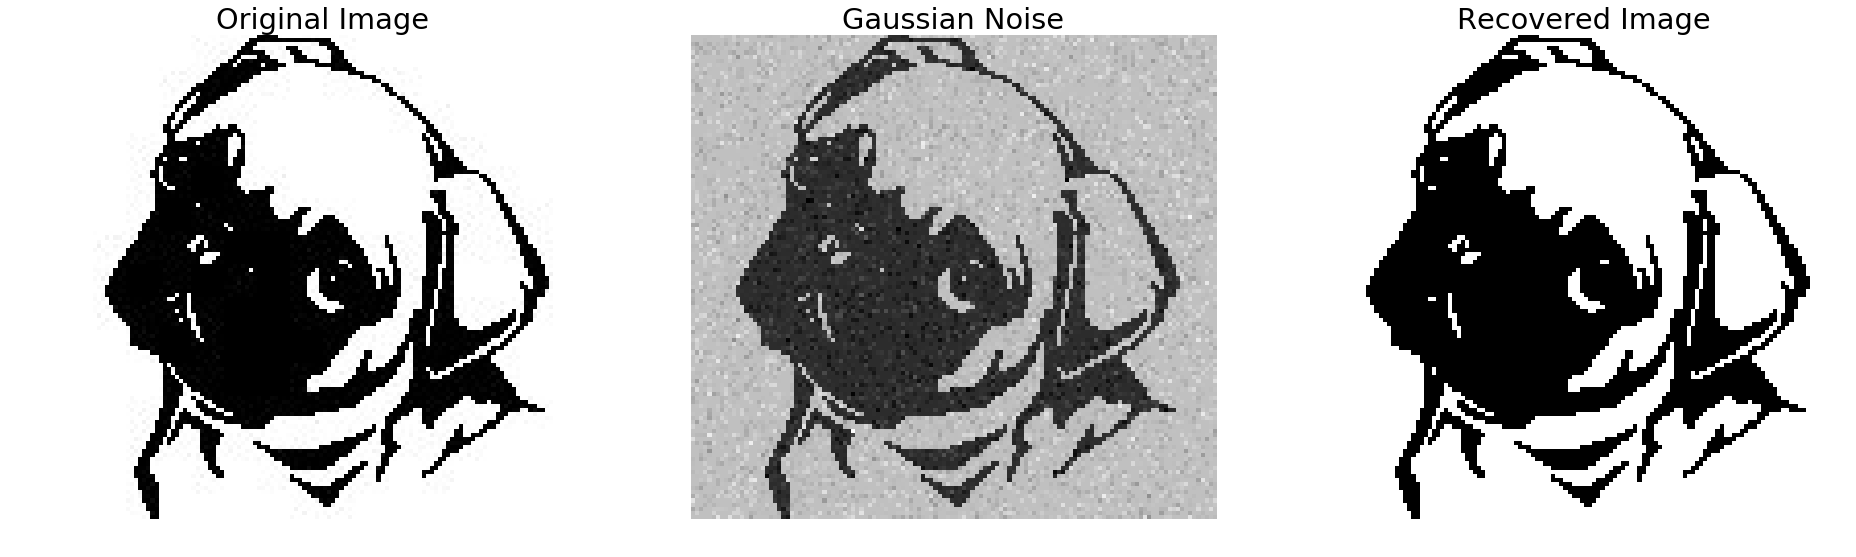
\includegraphics[width=0.3\linewidth]{q1noise05.png}\\
                    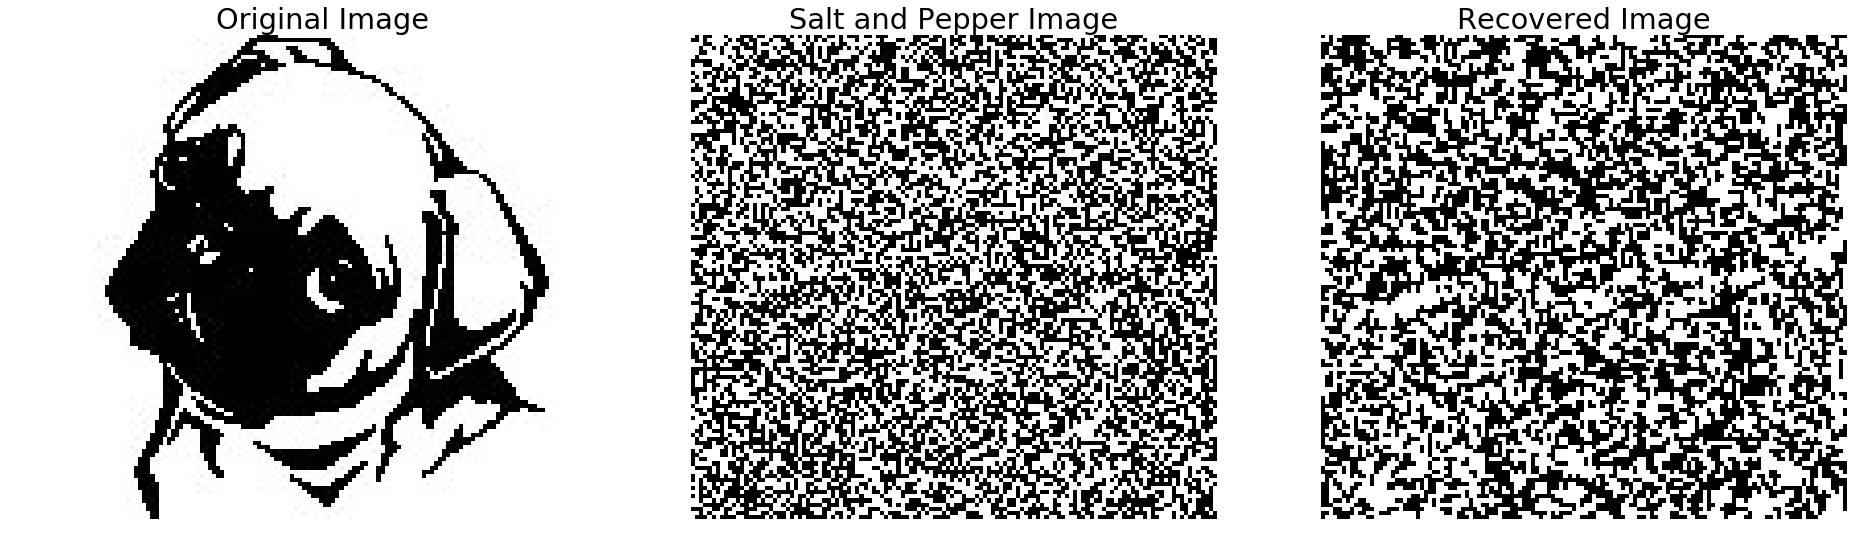
\includegraphics[width=0.3\linewidth]{q1noise05sp.png}
                \end{tabular}
            }
            \subfloat[][Noise proportion = 0.7]{
                \begin{tabular}{c}
                    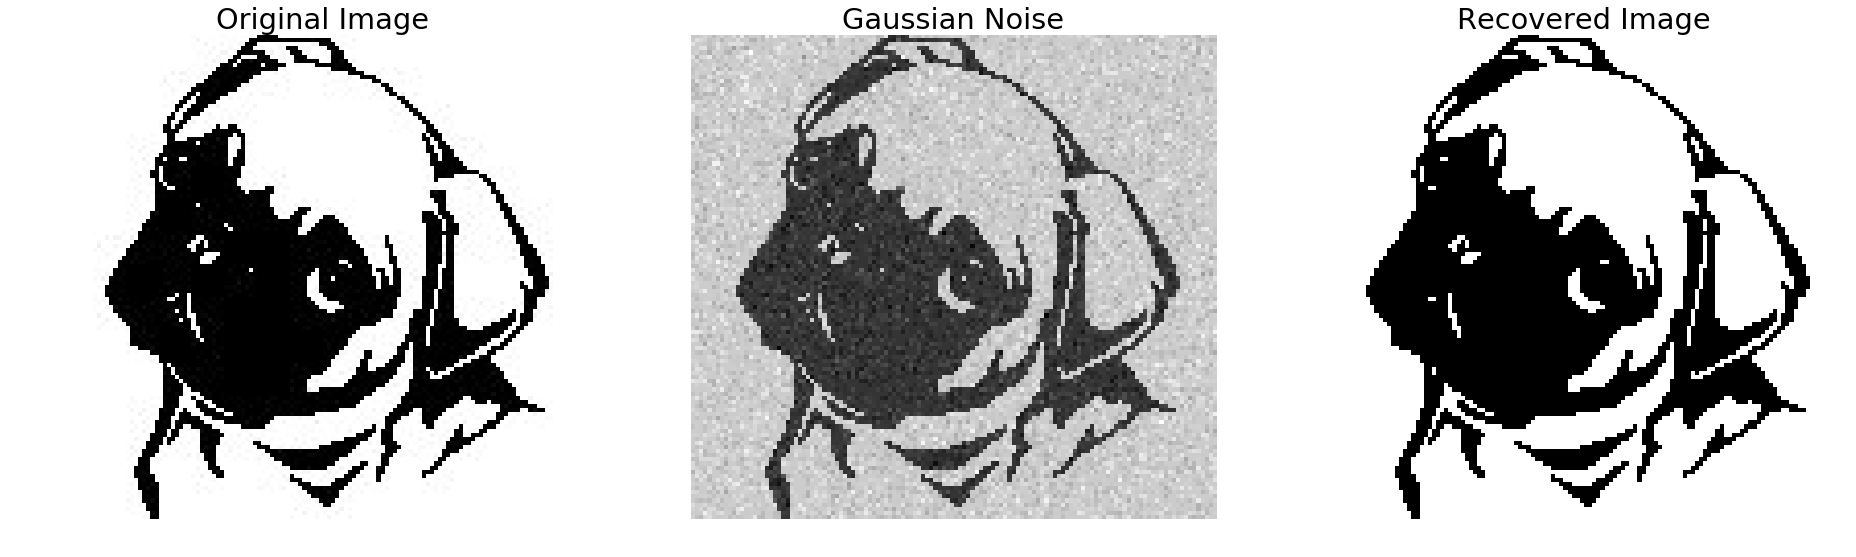
\includegraphics[width=0.3\linewidth]{output_3_1.png}\\
                    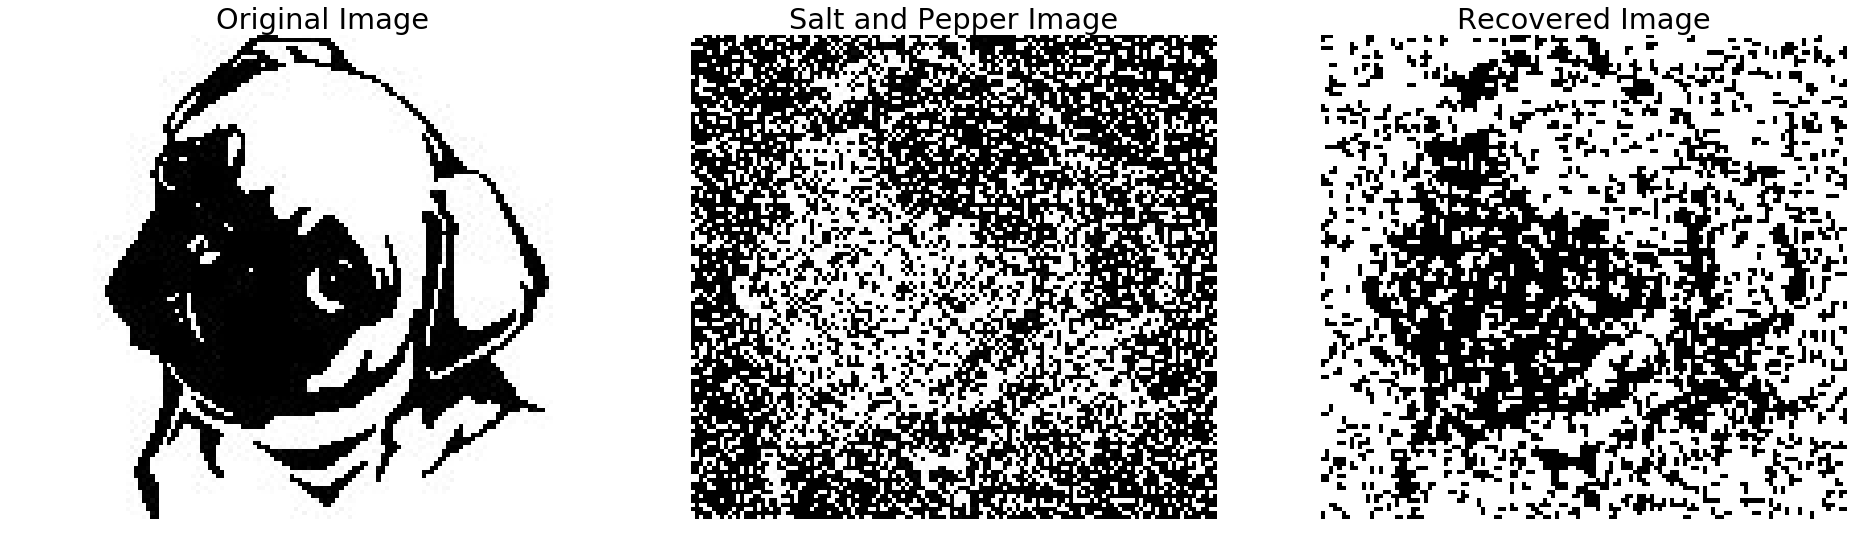
\includegraphics[width=0.3\linewidth]{output_3_3.png}
                \end{tabular}
            }
            \subfloat[][Noise proportion = 0.9]{
                \begin{tabular}{c}
                    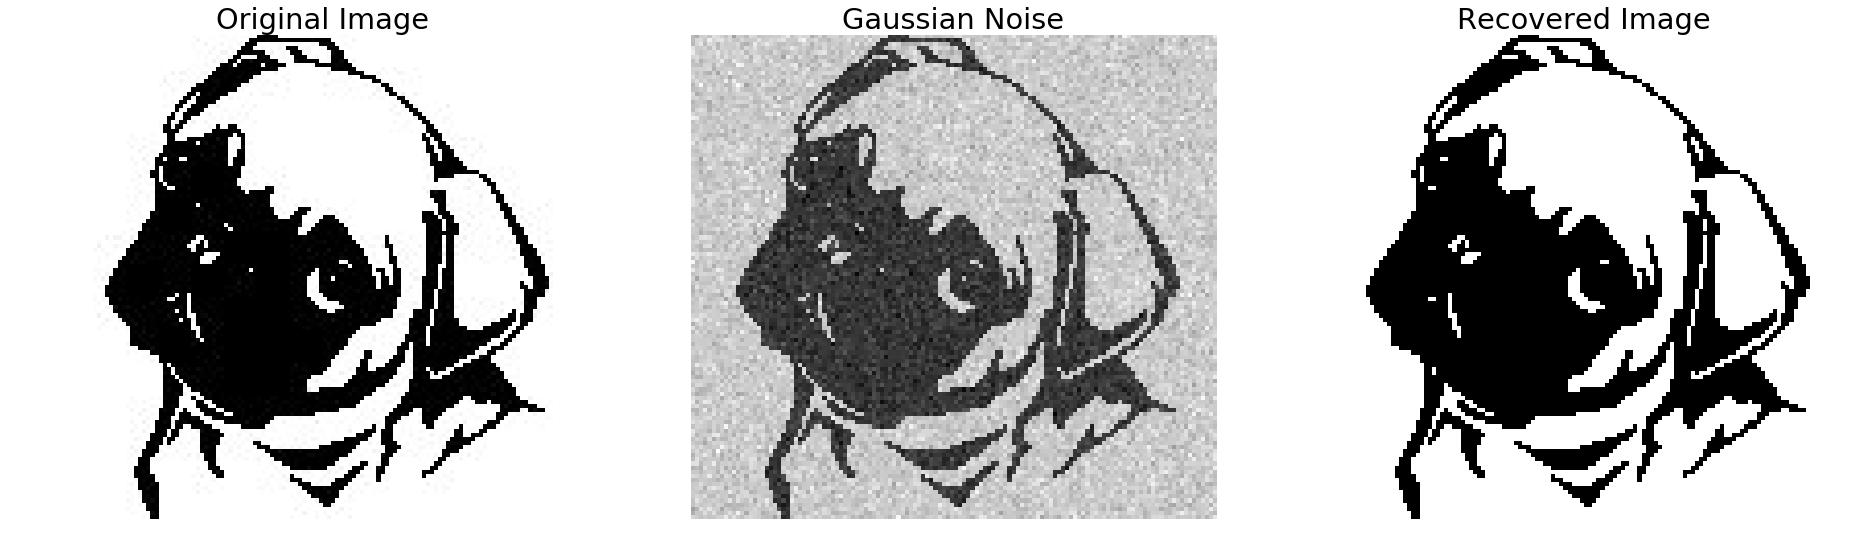
\includegraphics[width=0.3\linewidth]{q1noise09g.png}\\
                    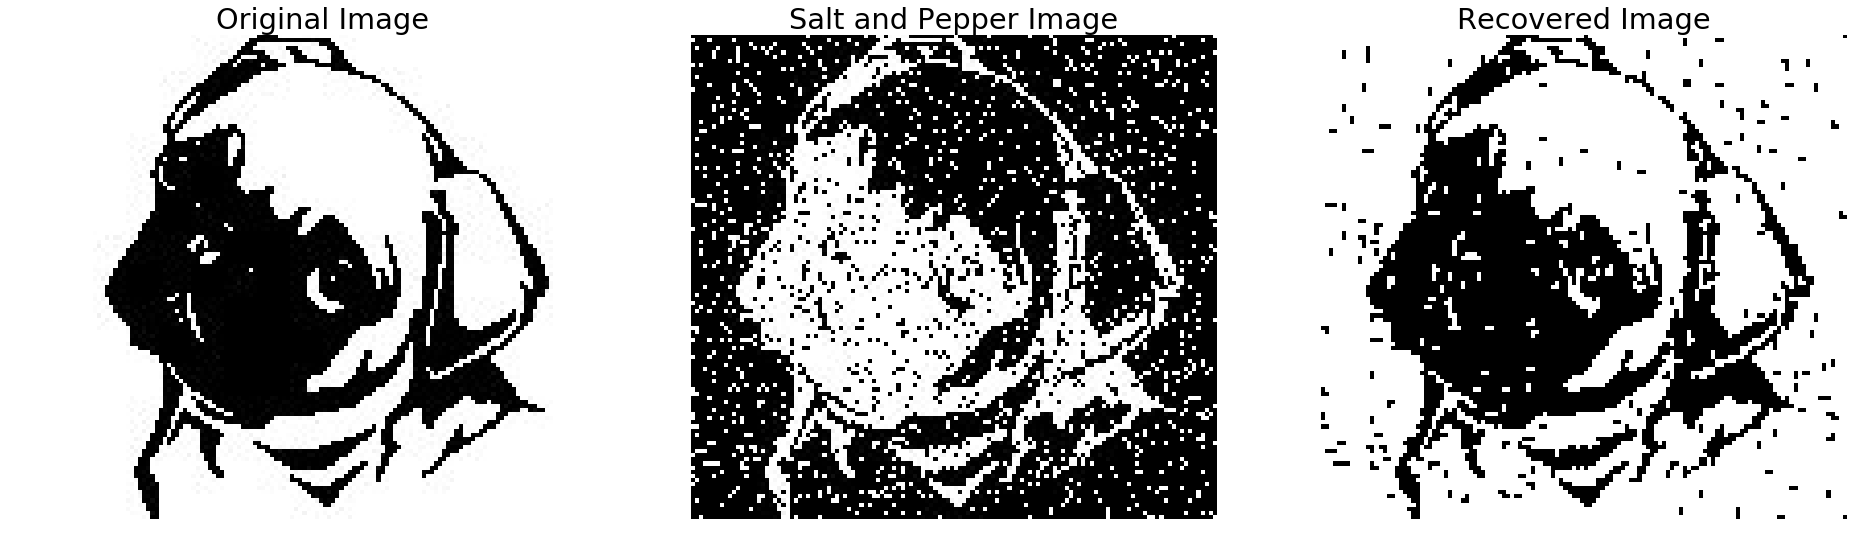
\includegraphics[width=0.3\linewidth]{q1noise09sp.png}
                \end{tabular}
            }
            \caption{Each subfigure from left to right shows, the original, one with added noise and the recovered image using ICM. The top is Gaussian noise, the bottom is salt \& pepper noise.}
            \label{fig:q1}
        \end{figure}
        \par
        The method takes 2 and 5 iterations respectively. For the salt and pepper image, this clearly still isn’t a "decent" image, but for the Gaussian, the image is very close to the original. The salt and pepper recovery varies the most, it's at its worst when half the pixels are altered. It performs better however towards the extremes (when either 0.9 or 0.1 is the proportion) since it's closer to the original (or the negative of the original). Recovery from Gaussian noise seems fairly consistent, irrespective of the amount.
        \begin{figure}[h]
            \centering
            \subfloat[][Noise proportion = 0.5]{
                \begin{tabular}{c}
                    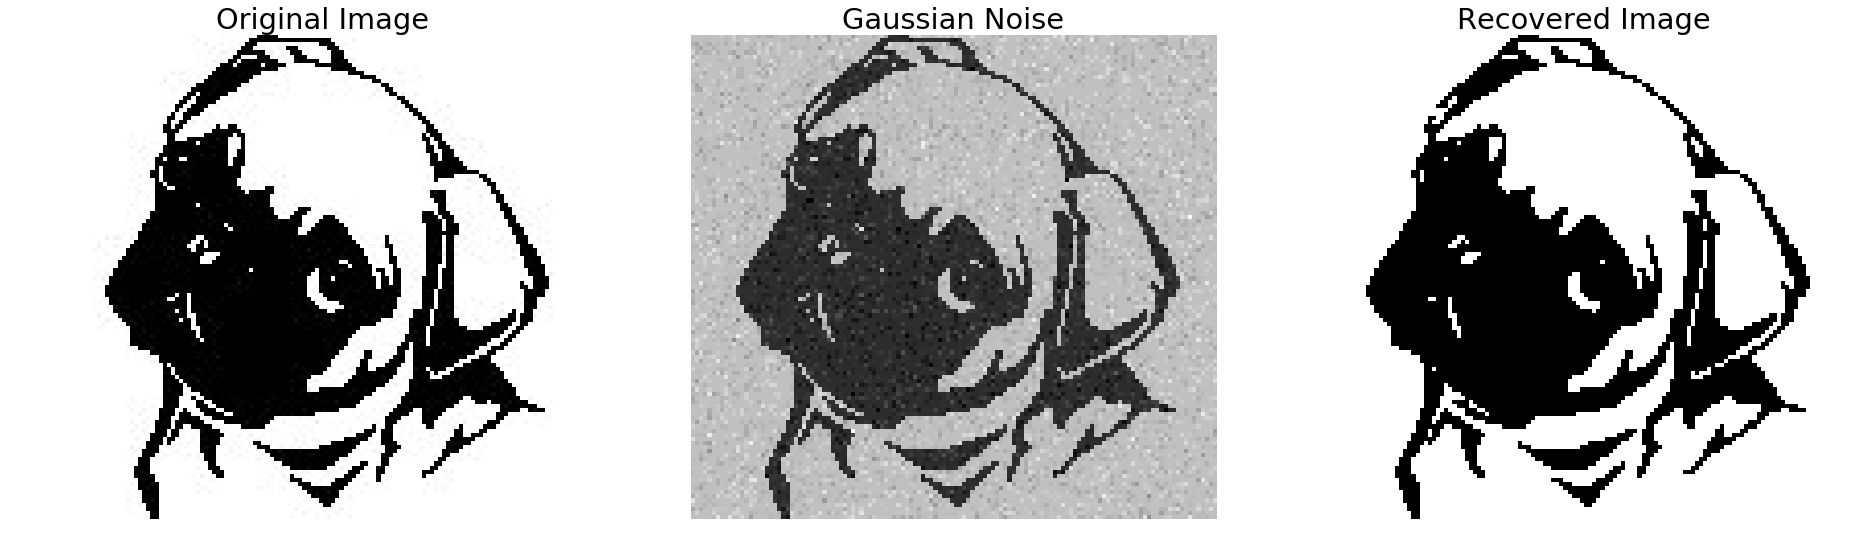
\includegraphics[width=0.3\linewidth]{q2noise05g.png}\\
                    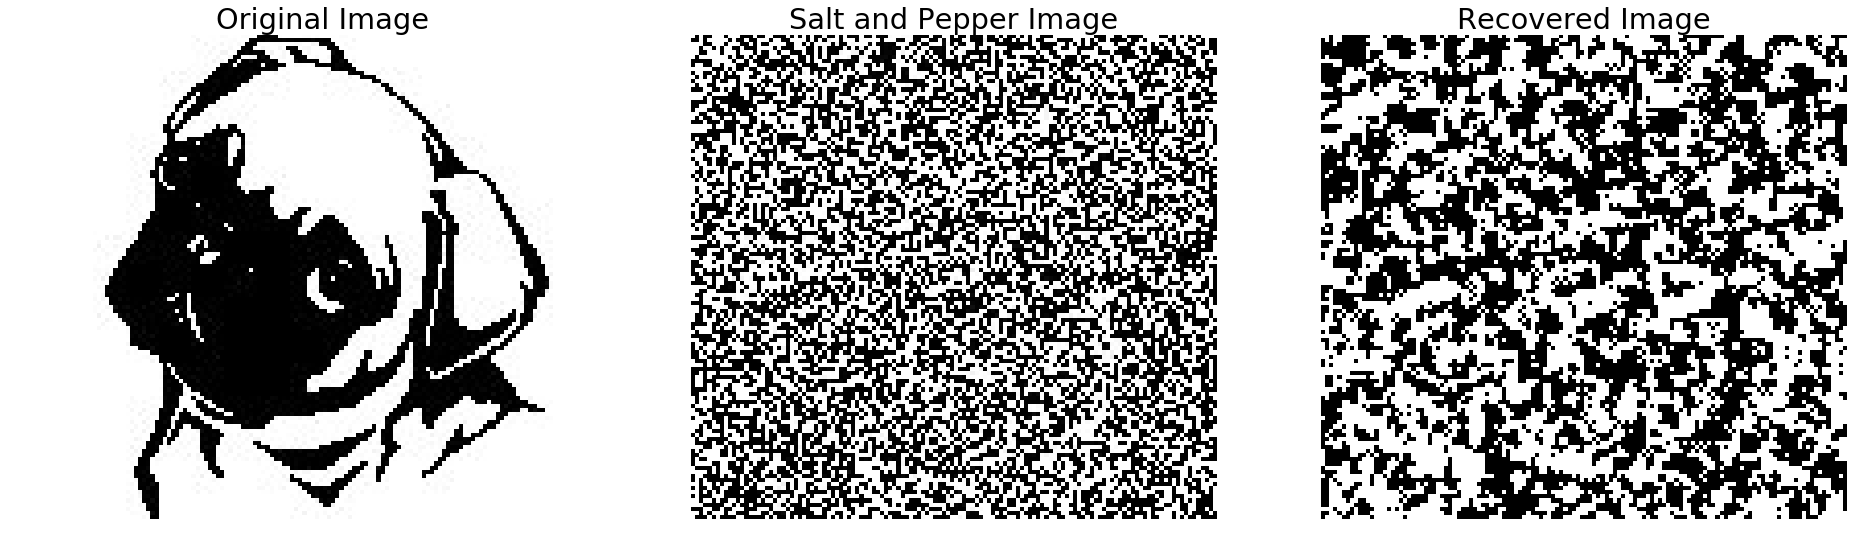
\includegraphics[width=0.3\linewidth]{q2noise05sp.png}
                \end{tabular}
            }
            \subfloat[][Noise proportion = 0.7]{
                \begin{tabular}{c}
                    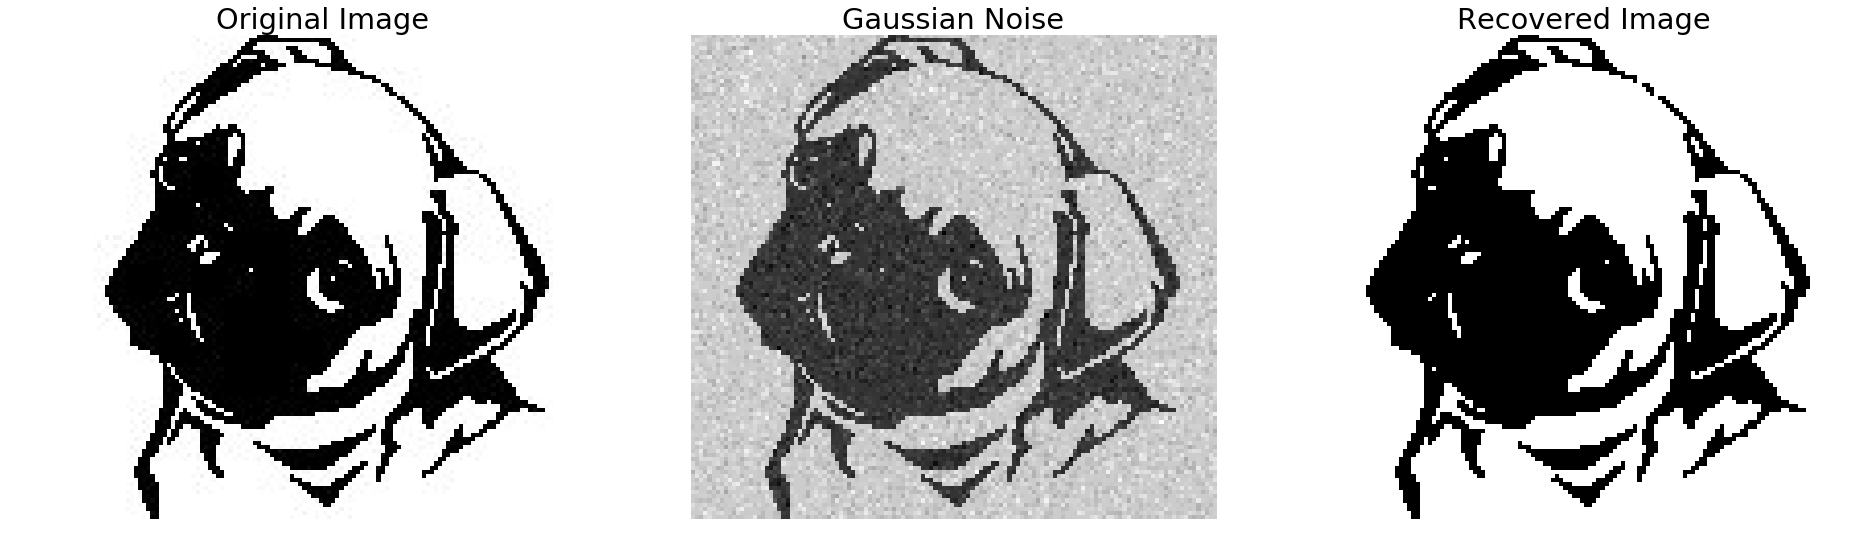
\includegraphics[width=0.3\linewidth]{output_7_0.png}\\
                    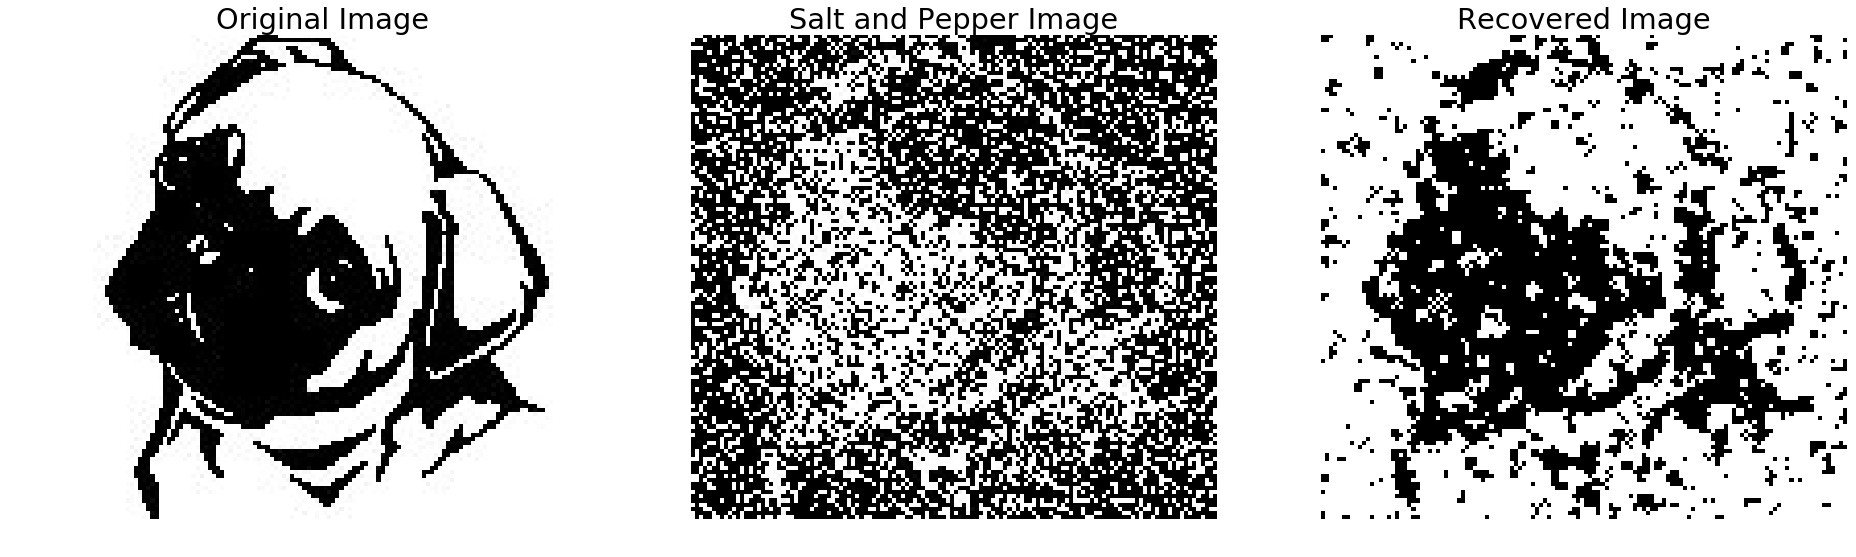
\includegraphics[width=0.3\linewidth]{output_7_2.png}
                \end{tabular}
            }
            \subfloat[][Noise proportion = 0.9]{
                \begin{tabular}{c}
                    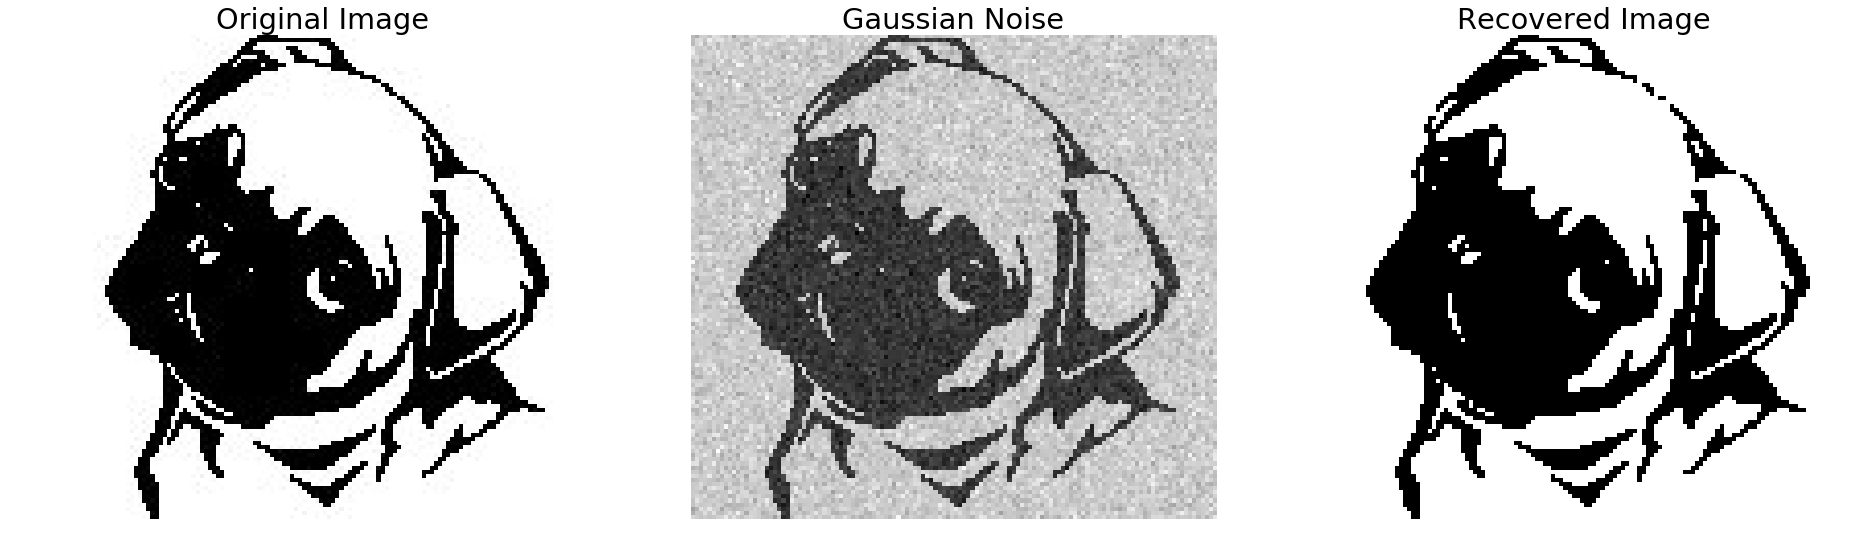
\includegraphics[width=0.3\linewidth]{q2noise09g.png}\\
                    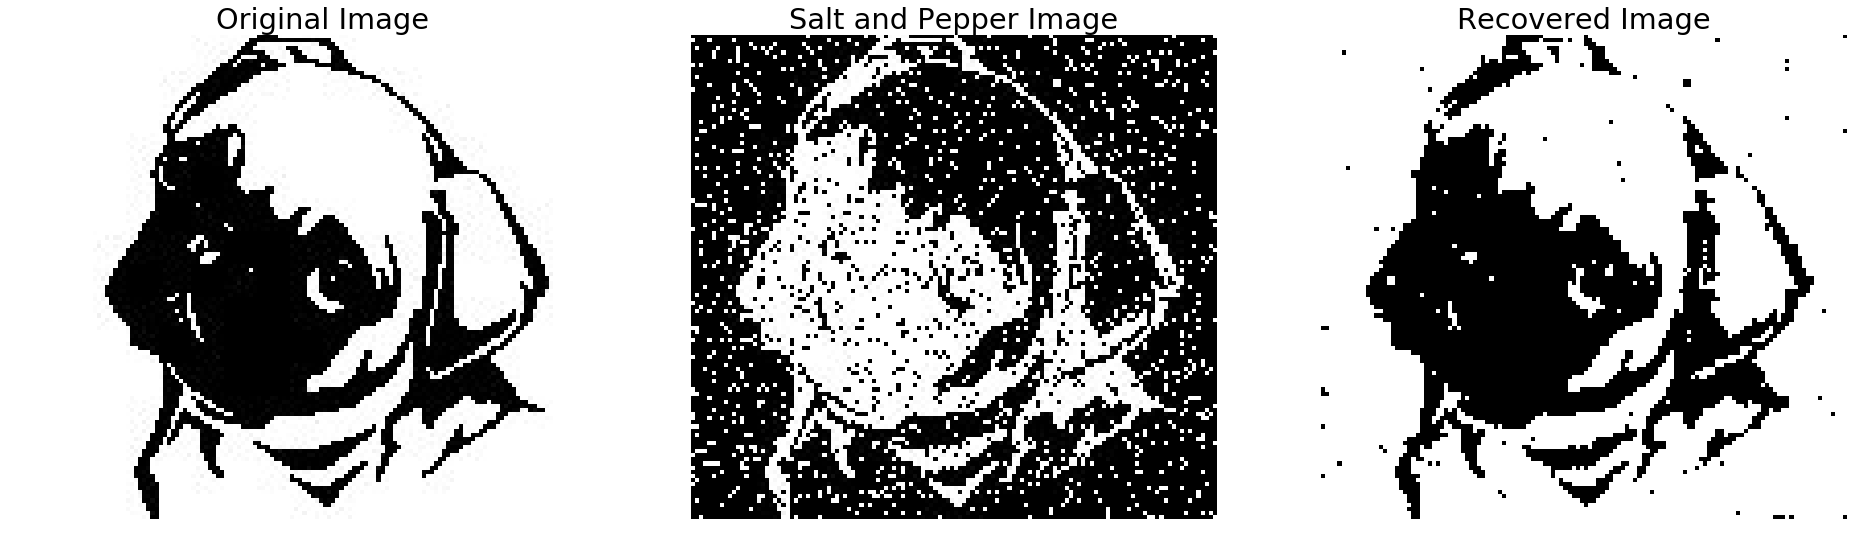
\includegraphics[width=0.3\linewidth]{q2noise09sp.png}
                \end{tabular}
            }
            \caption{Results of running Gibbs sampling approach.}
            \label{fig:q2}
        \end{figure}
    \section*{Question 2}
        \par
        As before the Gibbs approach produced better results for the Gaussian noise (shown in ~\ref{fig:q2}). It still wasn't able to recover the salt and pepper picture in (a), however produced better results for both the other salt and pepper images.
        \begin{figure}[h]
            \centering
            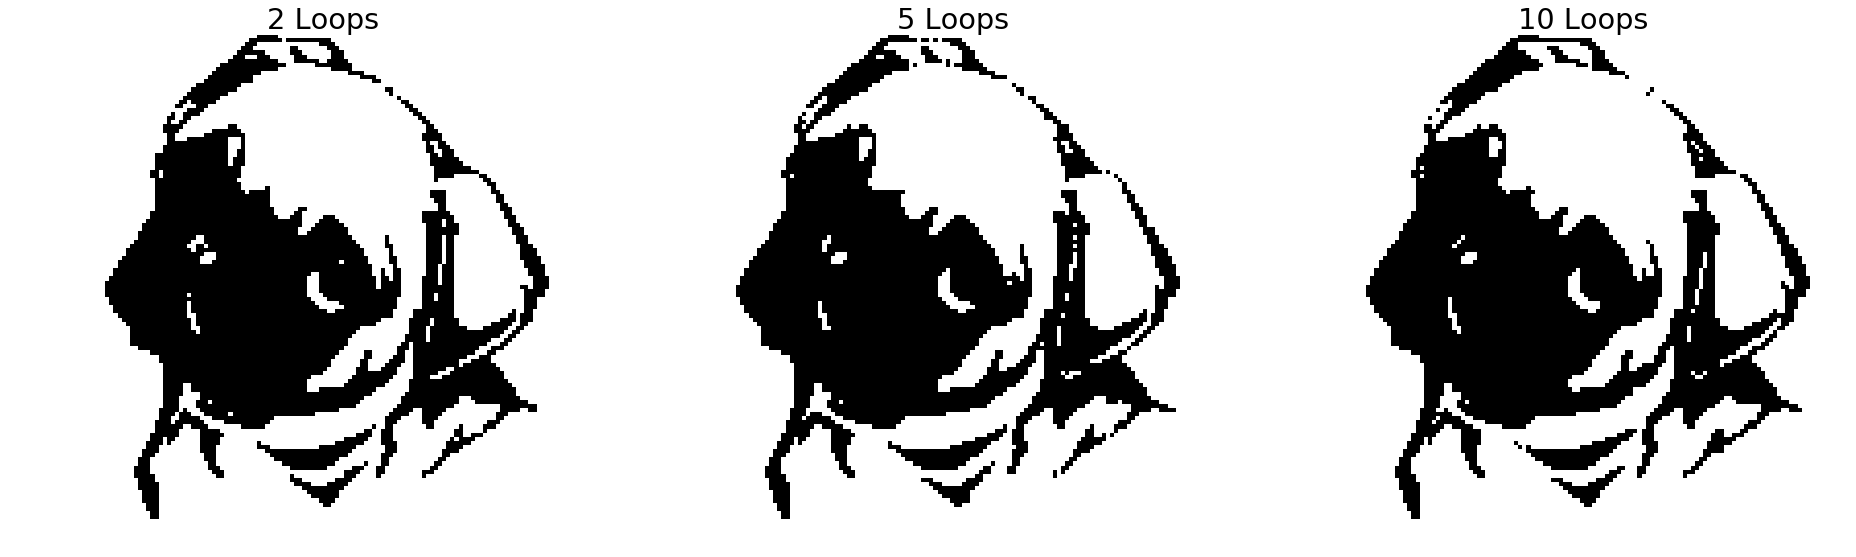
\includegraphics[width=0.5\linewidth]{output_7_1.png}
            \caption{Gibbs sampling for different iterations (2, 5 and 10 respectively).}
            \label{fig:q2a}
        \end{figure}
        \par
        Running the Gibbs sampler for more iterations seemed to have little impact on the overall result. If anything it may have slightly reduced the quality of the overall result.
    \section*{Question 3}
        \begin{figure}[h]
            \centering
            \subfloat[][Salt and pepper (top) and Gaussian (bottom)]{
                \begin{tabular}{c}
                    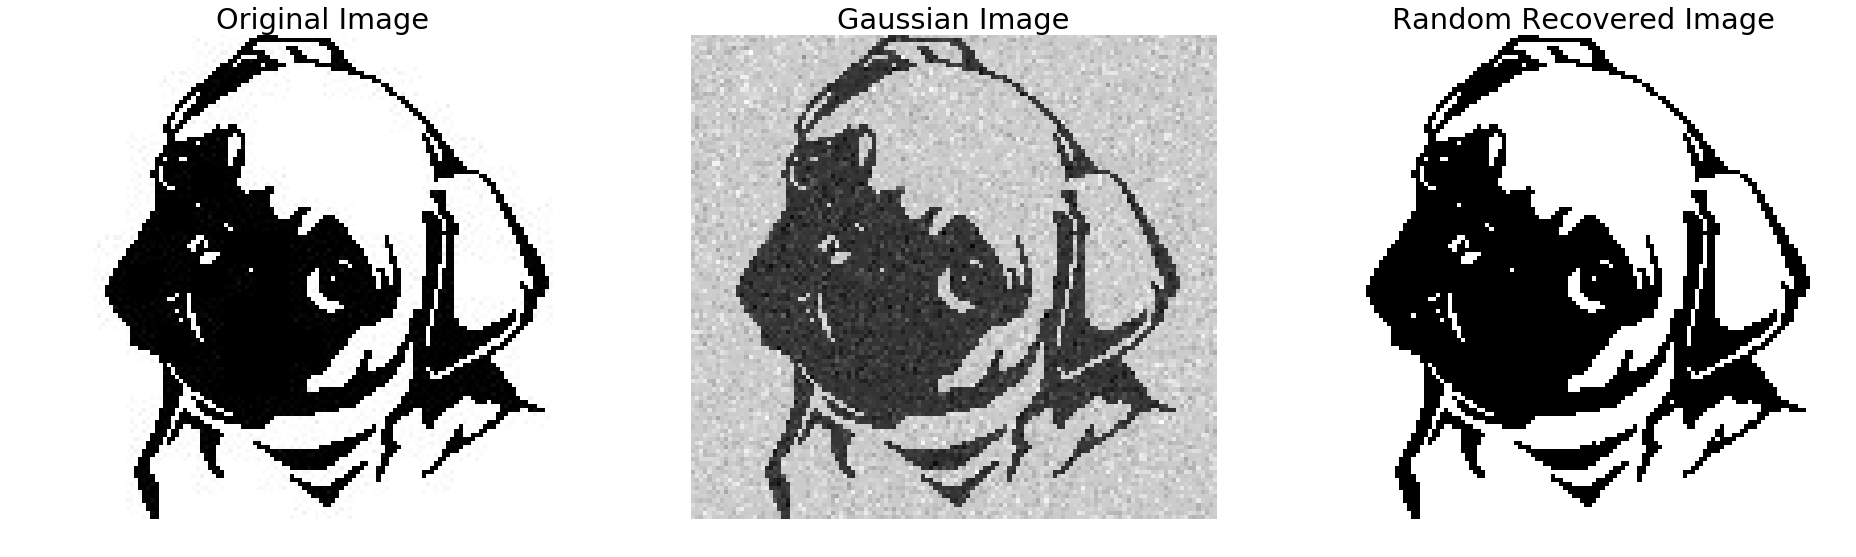
\includegraphics[width=0.5\linewidth]{output_8_1.png}\\
                    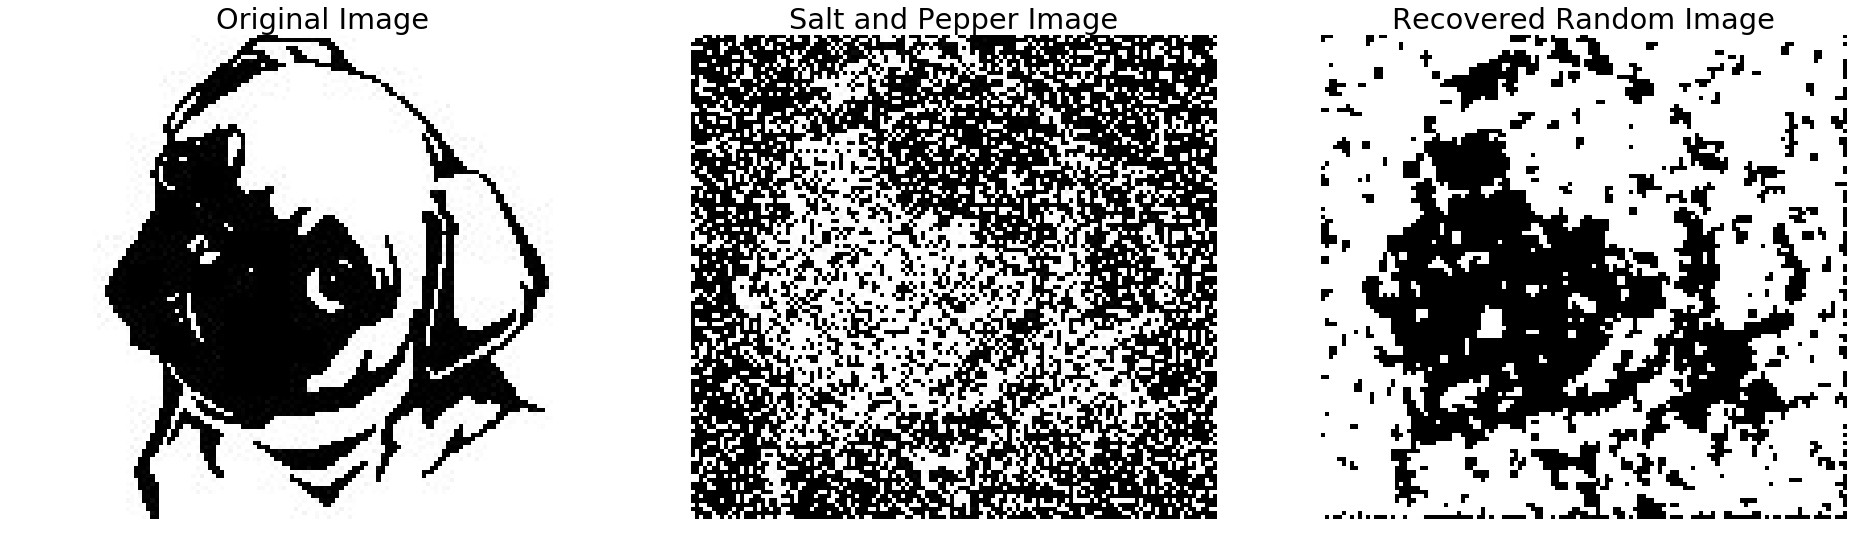
\includegraphics[width=0.5\linewidth]{output_8_5.png}
                \end{tabular}
            }
            \subfloat[][Gaussian after more iterations (10, 50, 100 resp.)]{
                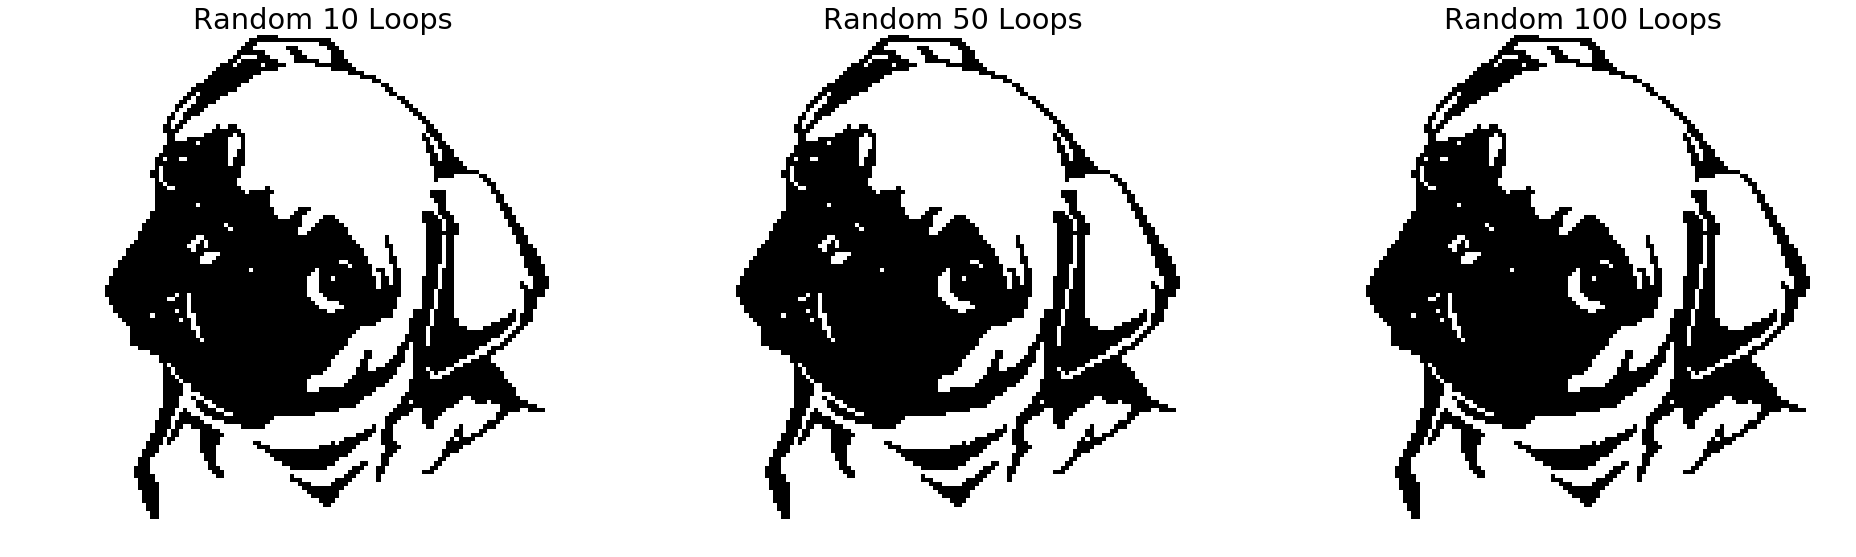
\includegraphics[width=0.5\linewidth]{output_8_3.png}
            }
            \caption{Random Gibbs sampling results.}
            \label{fig:q3}
        \end{figure}
        \par
        When looping randomly, the gaussian noise image seems to near enough recover the image perfectly
        in what appears to be one iteration, whilst the S\&P image seems to peak in quality at around
        the 500,000 iteration points. In this case, iterations are how many pixels are being updated.
    \section*{Question 4}
        \par
        As stated above, the image does not always improve, particularly with the salt and pepper image,
        after an optimal number of iterations, the image declines back into a less-recognisable mess. The
        gaussian example shows detrimental effects from looping more than a nice amount of times, as
        the image quality decreases the more loops are applied.

    \section*{Question 5}
    \par To reason about the difference between $KL(q(x)||p(x))$ and $KL(p(x)||q(x))$, we'll consider the specific case where we fix $p(x) = 0, q(x) > 0$. Using the definition of the KL Divergence, $KL(q(x)||p(x)) = \int q(x) log\frac{p(x)}{q(x)}$ we can compute that $$\lim_{p(x)\rightarrow 0}\, q(x) log \frac{p(x)}{q(x)} = -\infty$$ This would mean that if there is some region where we assign probability mass in $q(x)$ that $p(x)$ assigns no probability mass to, then the KL divergence will be of magnitude $\infty$.
    
    \par On the otherhand, if we fix $p(x), q(x)$ as before, and calculate $KL(p(x)||q(x))$ we get a very different result. $$\lim_{p(x)\rightarrow 0} \, p(x) log \frac{q(x)}{p(x)} = 0$$ What this suggests is that if there is probability mass at q(x), but none at p(x), it doesn't make a difference to the disimilarity. Clearly we should only be interested in either $KL(q(x)||p(x))$ or $KL(p(x)||q(x))$ since the two (at least in this extreme case) tell us different information.
    
    \par Let's say $q(x)$ is a distribution based off emperical evidence and $p(x)$ is our model and we fix the values as before, then $KL(q(x)||p(x)) = \infty$. Intuitively this makes sense, if a region in the model has 0 probability mass and yet the evidence places probability mass there, it seems sensible to say the model is disimilar to the evidence and that it should be rejected. The alternative, makes little sense when treating $p(x)$ as a model and q(x) as evidence. We saw before that the evidence $q(x)$ placing probability mass where there is none in the model p(x) doesn't increase (or change) the KL divergence which seems wrong. 
    
    \par Taking that $KL(q(x)||p(x))$ is more useful for our purposes, we can also look at the example where $p(x)>0, q(x)=0$. In that case, we have $\lim_{q(x)\rightarrow 0} \, q(x) log \frac{p(x)}{q(x)} = 0$. This also makes sense, just because none of our evidence resulted in probability mass at that point, it doesn't mean our model is wrong. 
    
    \par A way you can think of this is if we made the statement "all pugs have red collars", the observation of just one pug without a red collar refutes that statement (ie the case where $KL(q(x)||p(x))=\infty$). On the otherhand, if we made the statement that "some pugs wear red collars" and didn't see any wearing red collars, we can't refute that statement (ie the case where $KL(q(x)||p(x))=0$). \cite{inftheory}
    
    \section*{Question 6}
        \begin{figure}[h]
            \centering
            \begin{tabular}{c}
                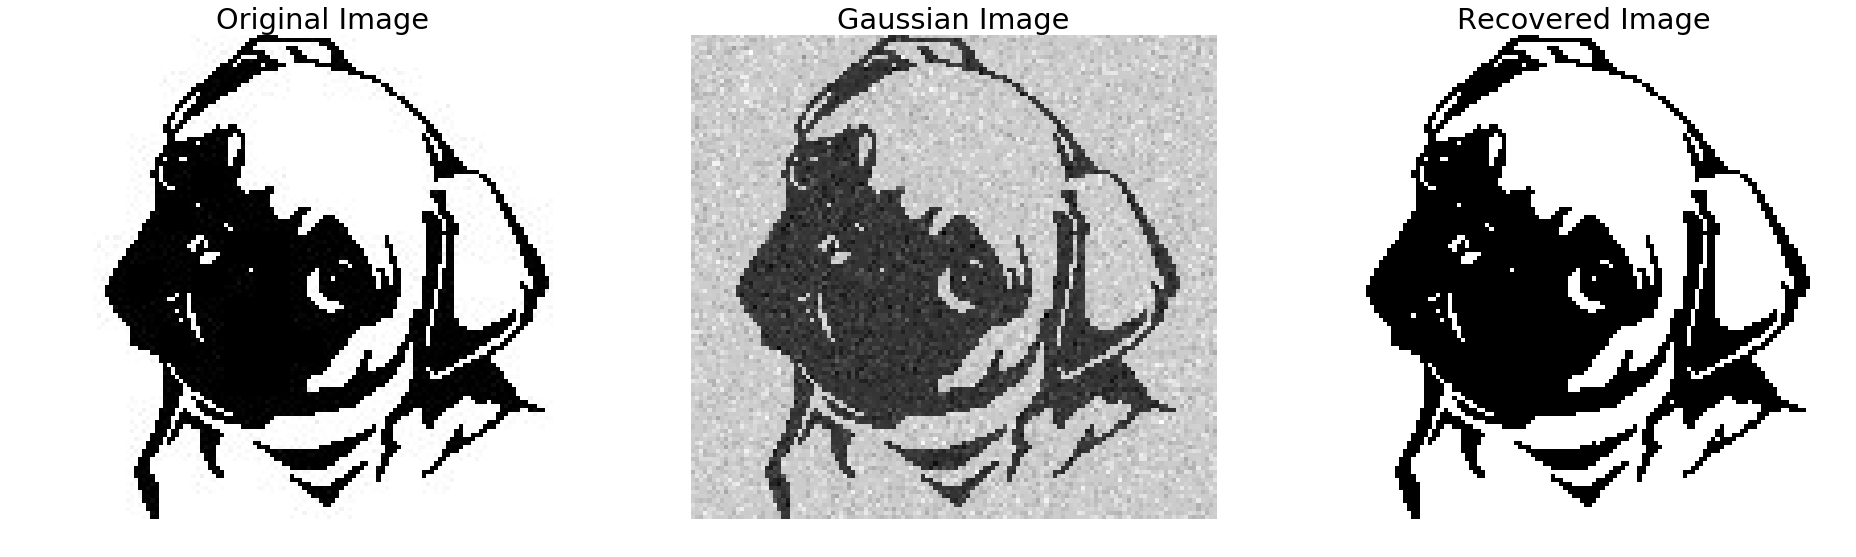
\includegraphics[width=0.5\linewidth]{output_10_0.png}\\
                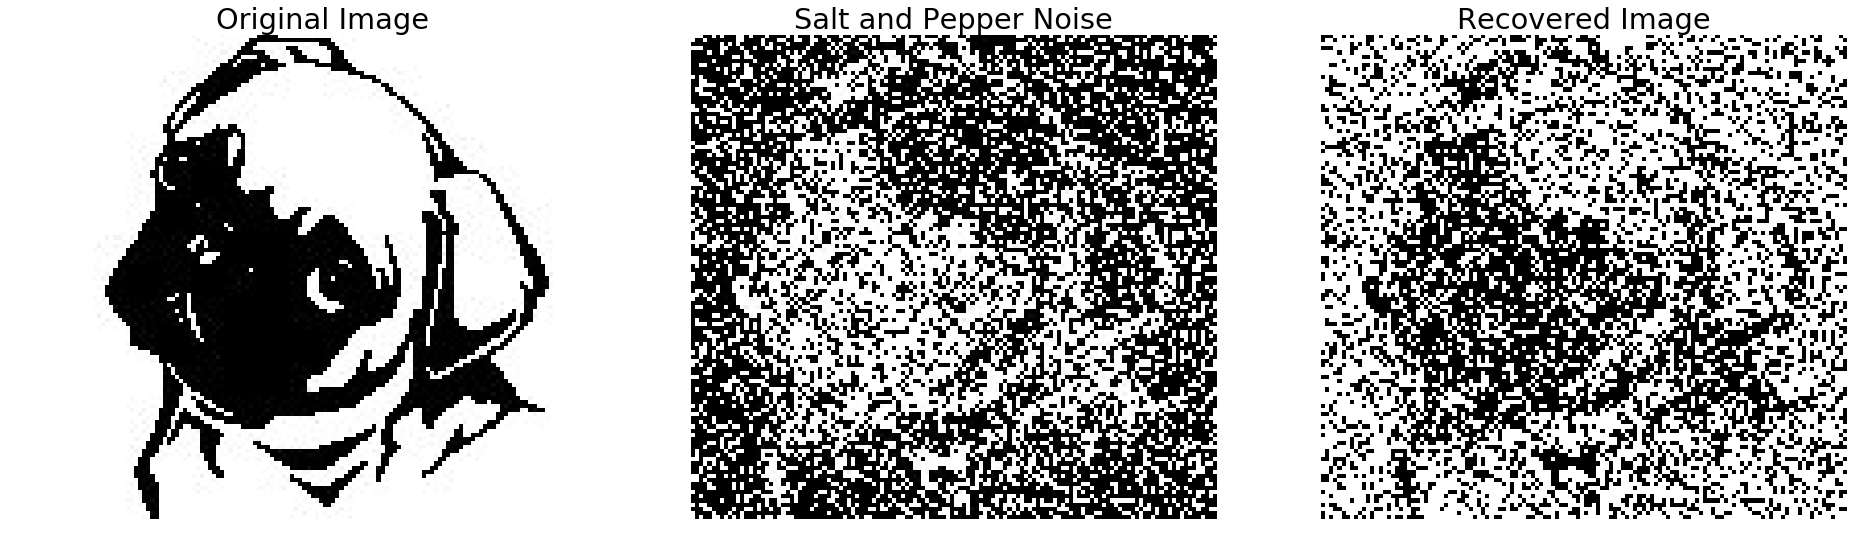
\includegraphics[width=0.5\linewidth]{output_10_1.png}
            \end{tabular}
            \caption{Results of Variational Bayes method}
            \label{fig:q6}
        \end{figure}
        \par The results for this are shown in figure ~\ref{fig:q6}.

    \section*{Question 7}
        \par The variational bayes method, as with the others, produces a good quality retrieval of the Gaussian image, but unlike the others, produces a fairly cleaner S\&P image.
    \section*{Question 8}
    \begin{figure}[h]
        \centering
        \begin{tabular}{c}
            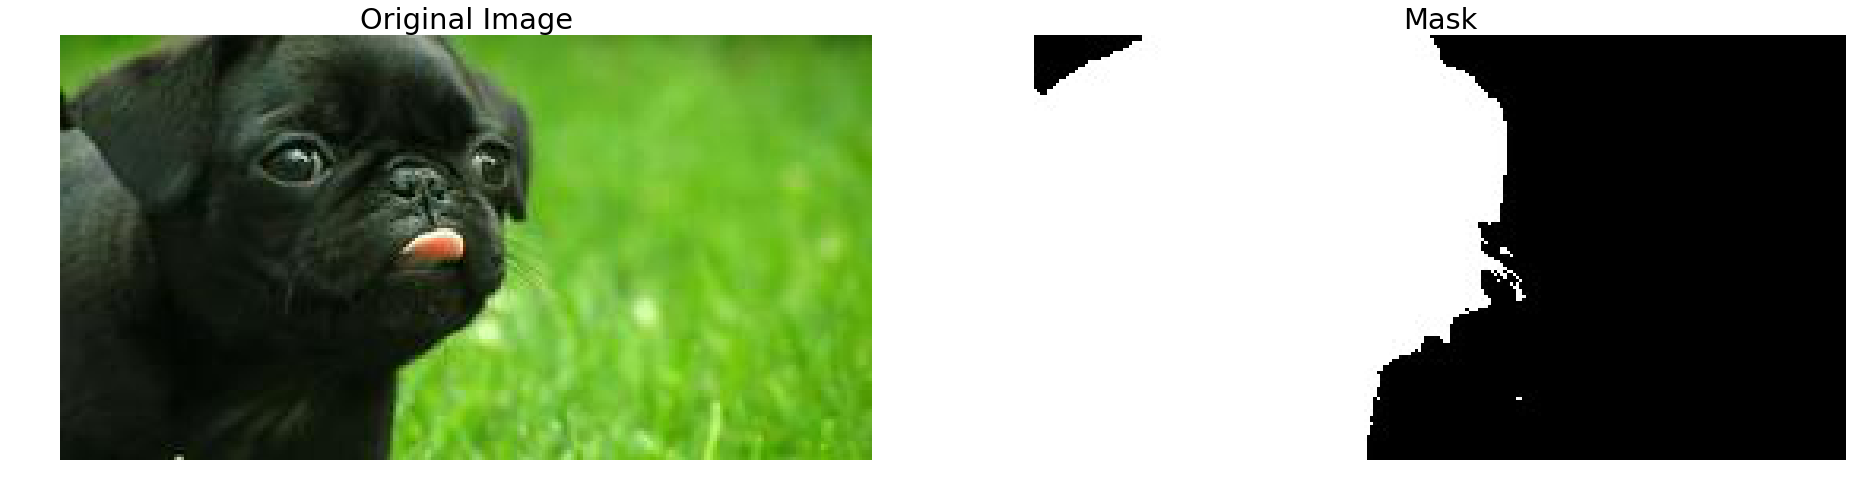
\includegraphics[width=0.5\linewidth]{output_12_1.png}\\
            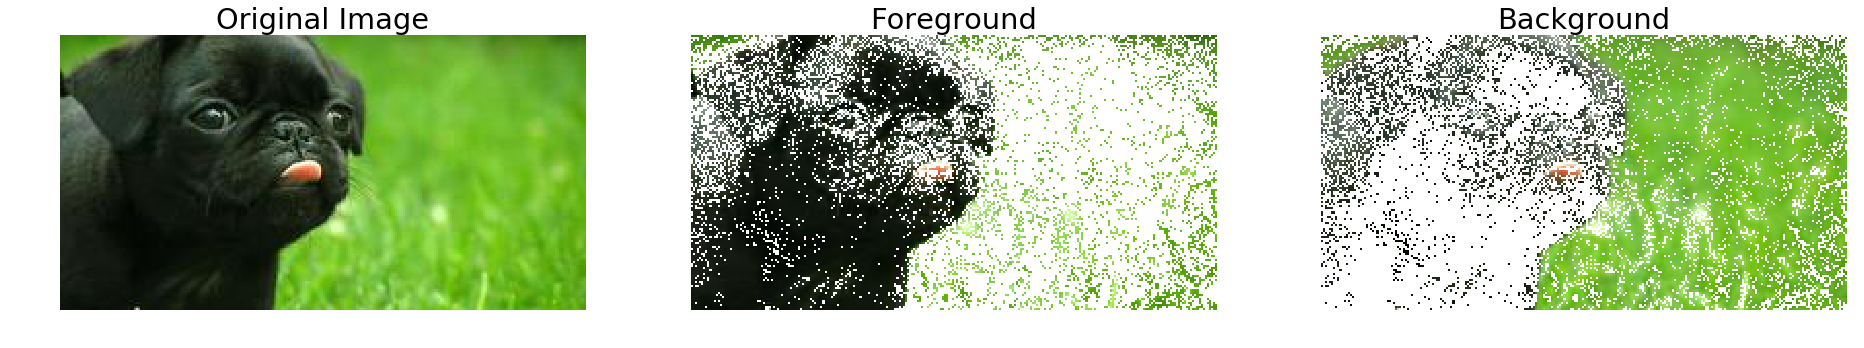
\includegraphics[width=0.5\linewidth]{output_14_0.png}
        \end{tabular}
        \caption{Results of image segmentation using Mean Field Variational Bayes method.}
        \label{fig:q8}
    \end{figure}
    \par The results for this are shown in figure ~\ref{fig:q8}.
    \section*{Question 9}
        \par The VAE model has two parts, an encoding part and decoding part. The encoding step uses a
        neural network to approximate the function that can “compress” the data into a latent variable (z
        in the given code). The decoding step makes use of the parameters learned by the encoding to take
        an input that represents the desired image as its latent variable and returns the image. The special
        feature of a Variational Autoencoder is that the latent variable is constrained to be a Gaussian
        distribution. This factors into the loss function as it takes into account both the KL divergence of the latent variable distribution and a unit Gaussian, and the difference between the original image
        and generated image. It also makes use of the reparameterization trick and represents the latent
        variable as the mean and standard deviation of it’s distribution instead of real values so that it
        can optimise the model using gradient descent. This is useful in image denoising as we could
        potentially use the encoding step to get the latent variable representation of the noisy image and
        then use the decoder to generate a denoised image. The difference between VAE and Variational
        Bayes is that VAE can learn to generate different images based on the different latent variables.
    \section*{Question 10}
        \begin{figure}[h]
            \centering
            \subfloat[][n = 0]{
                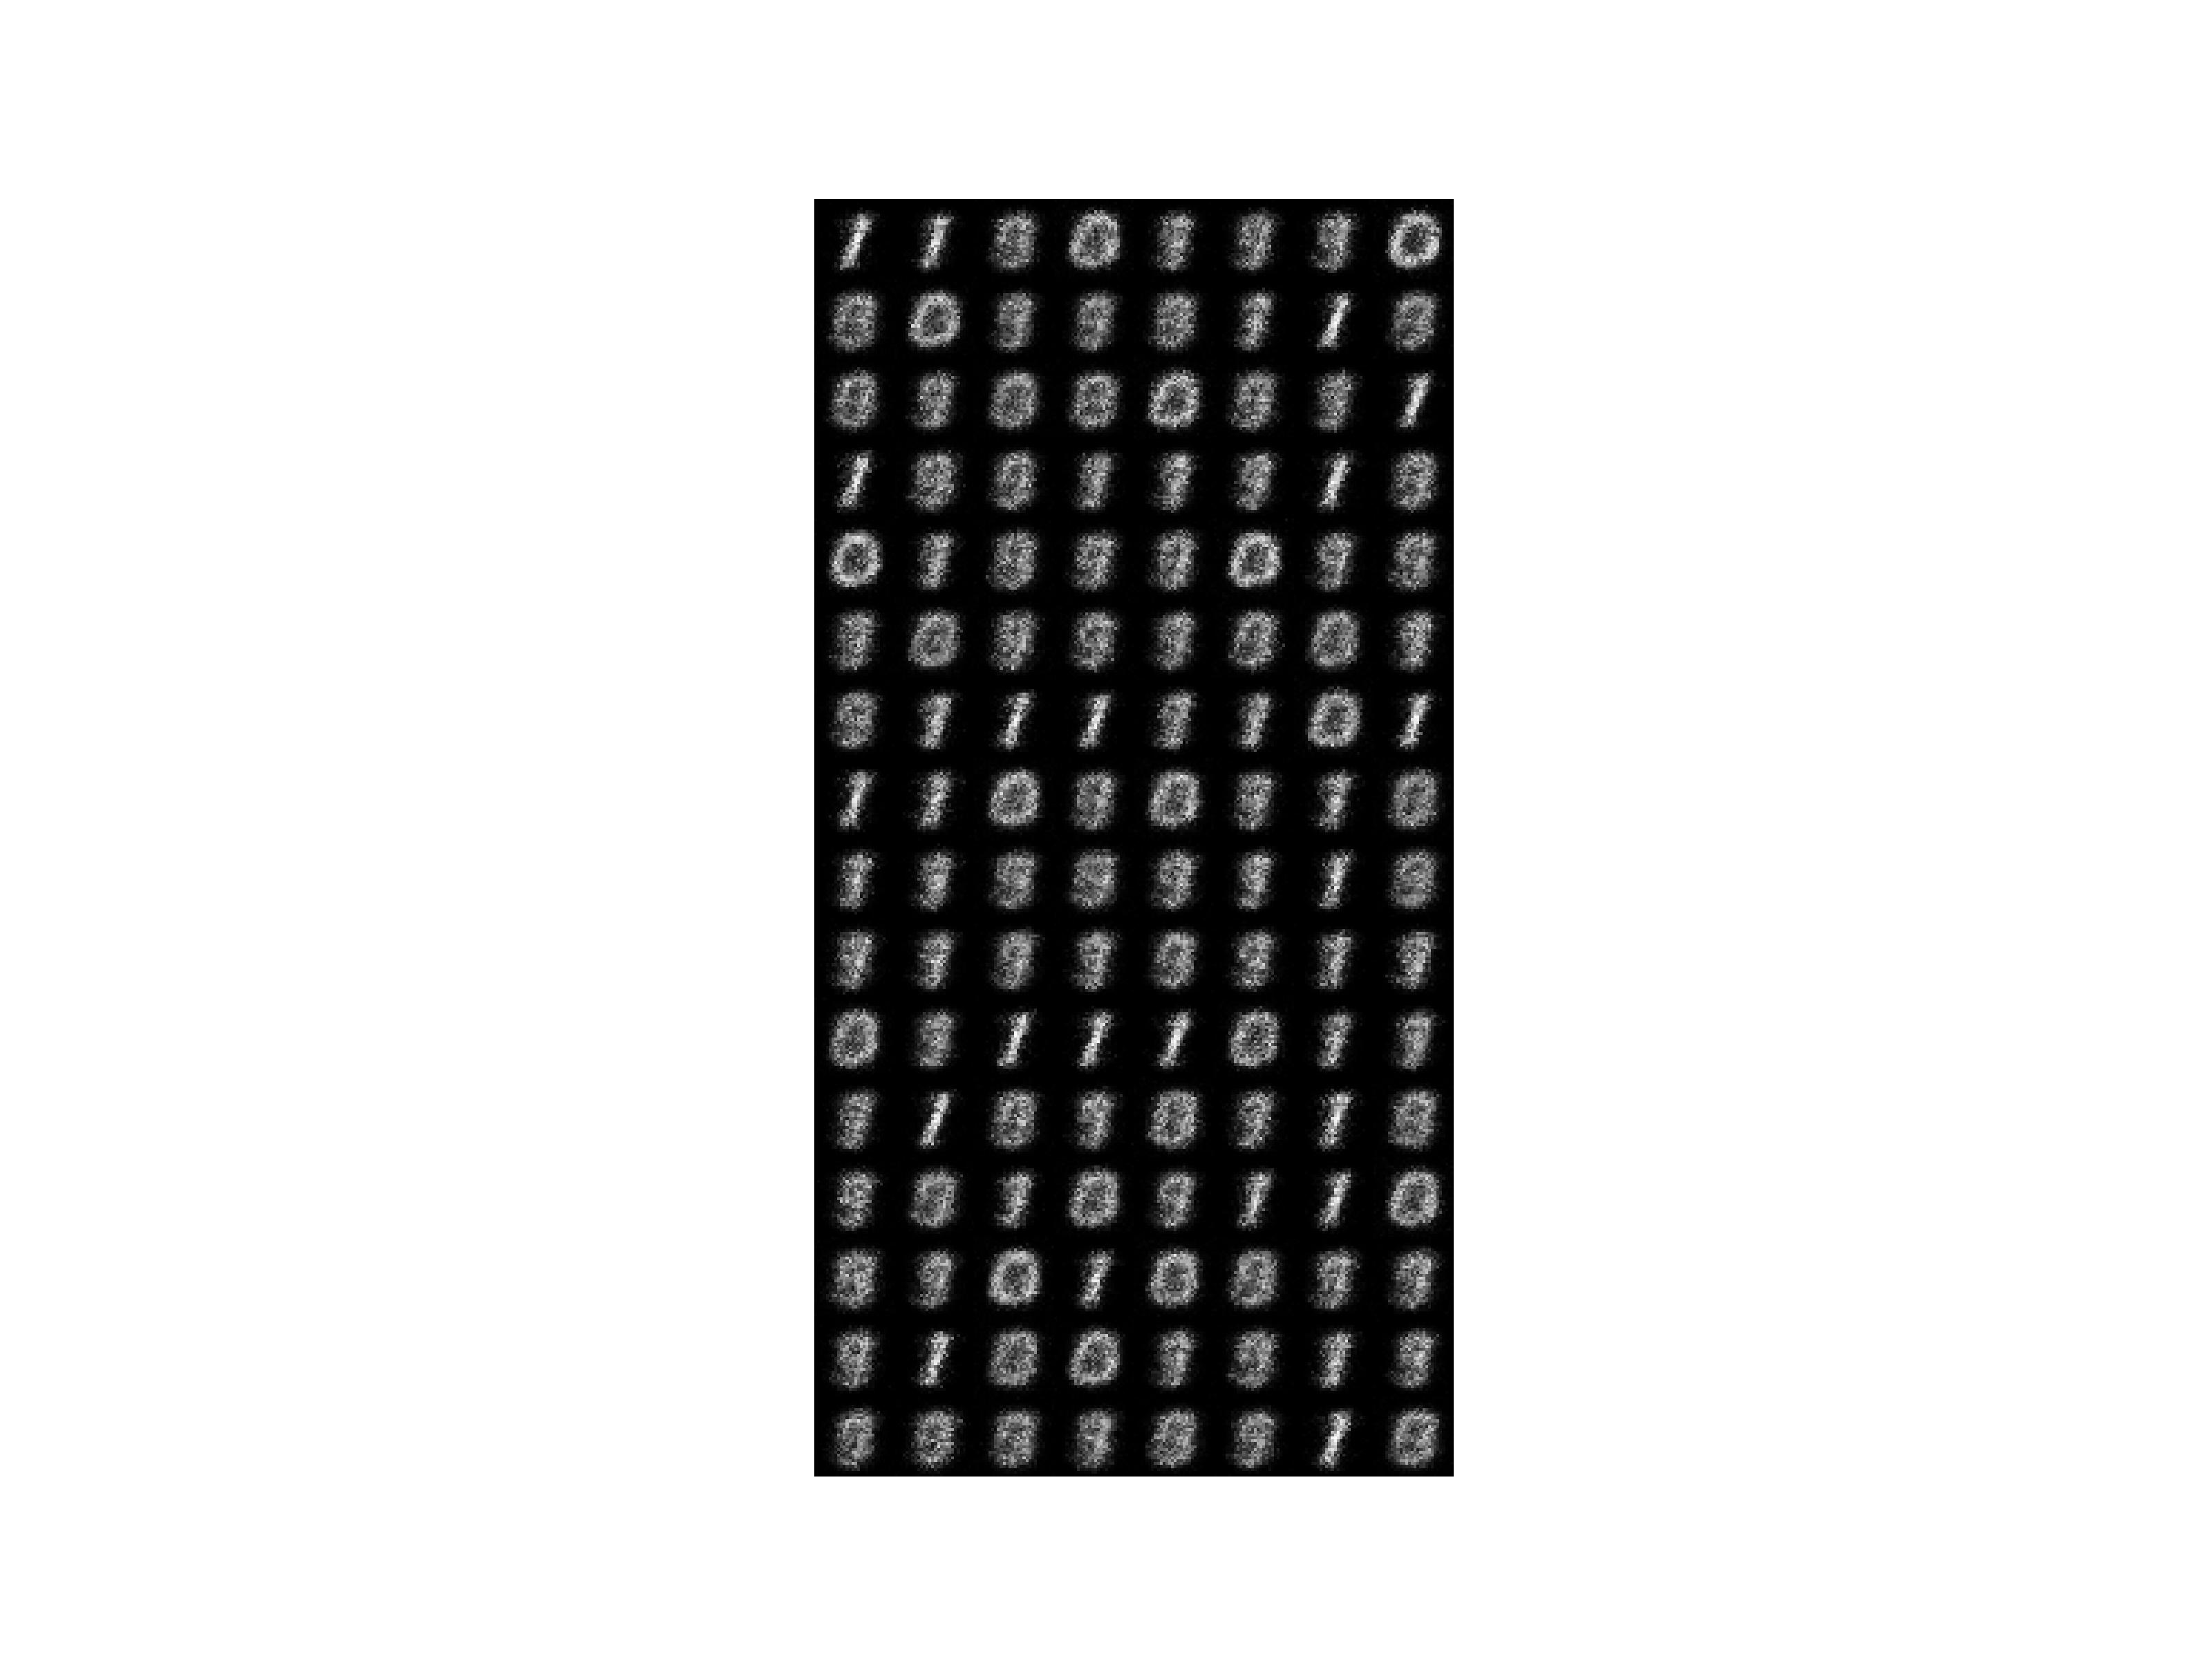
\includegraphics[width=0.3\linewidth]{plt0.png}
            }
            \subfloat[][n = 50]{
                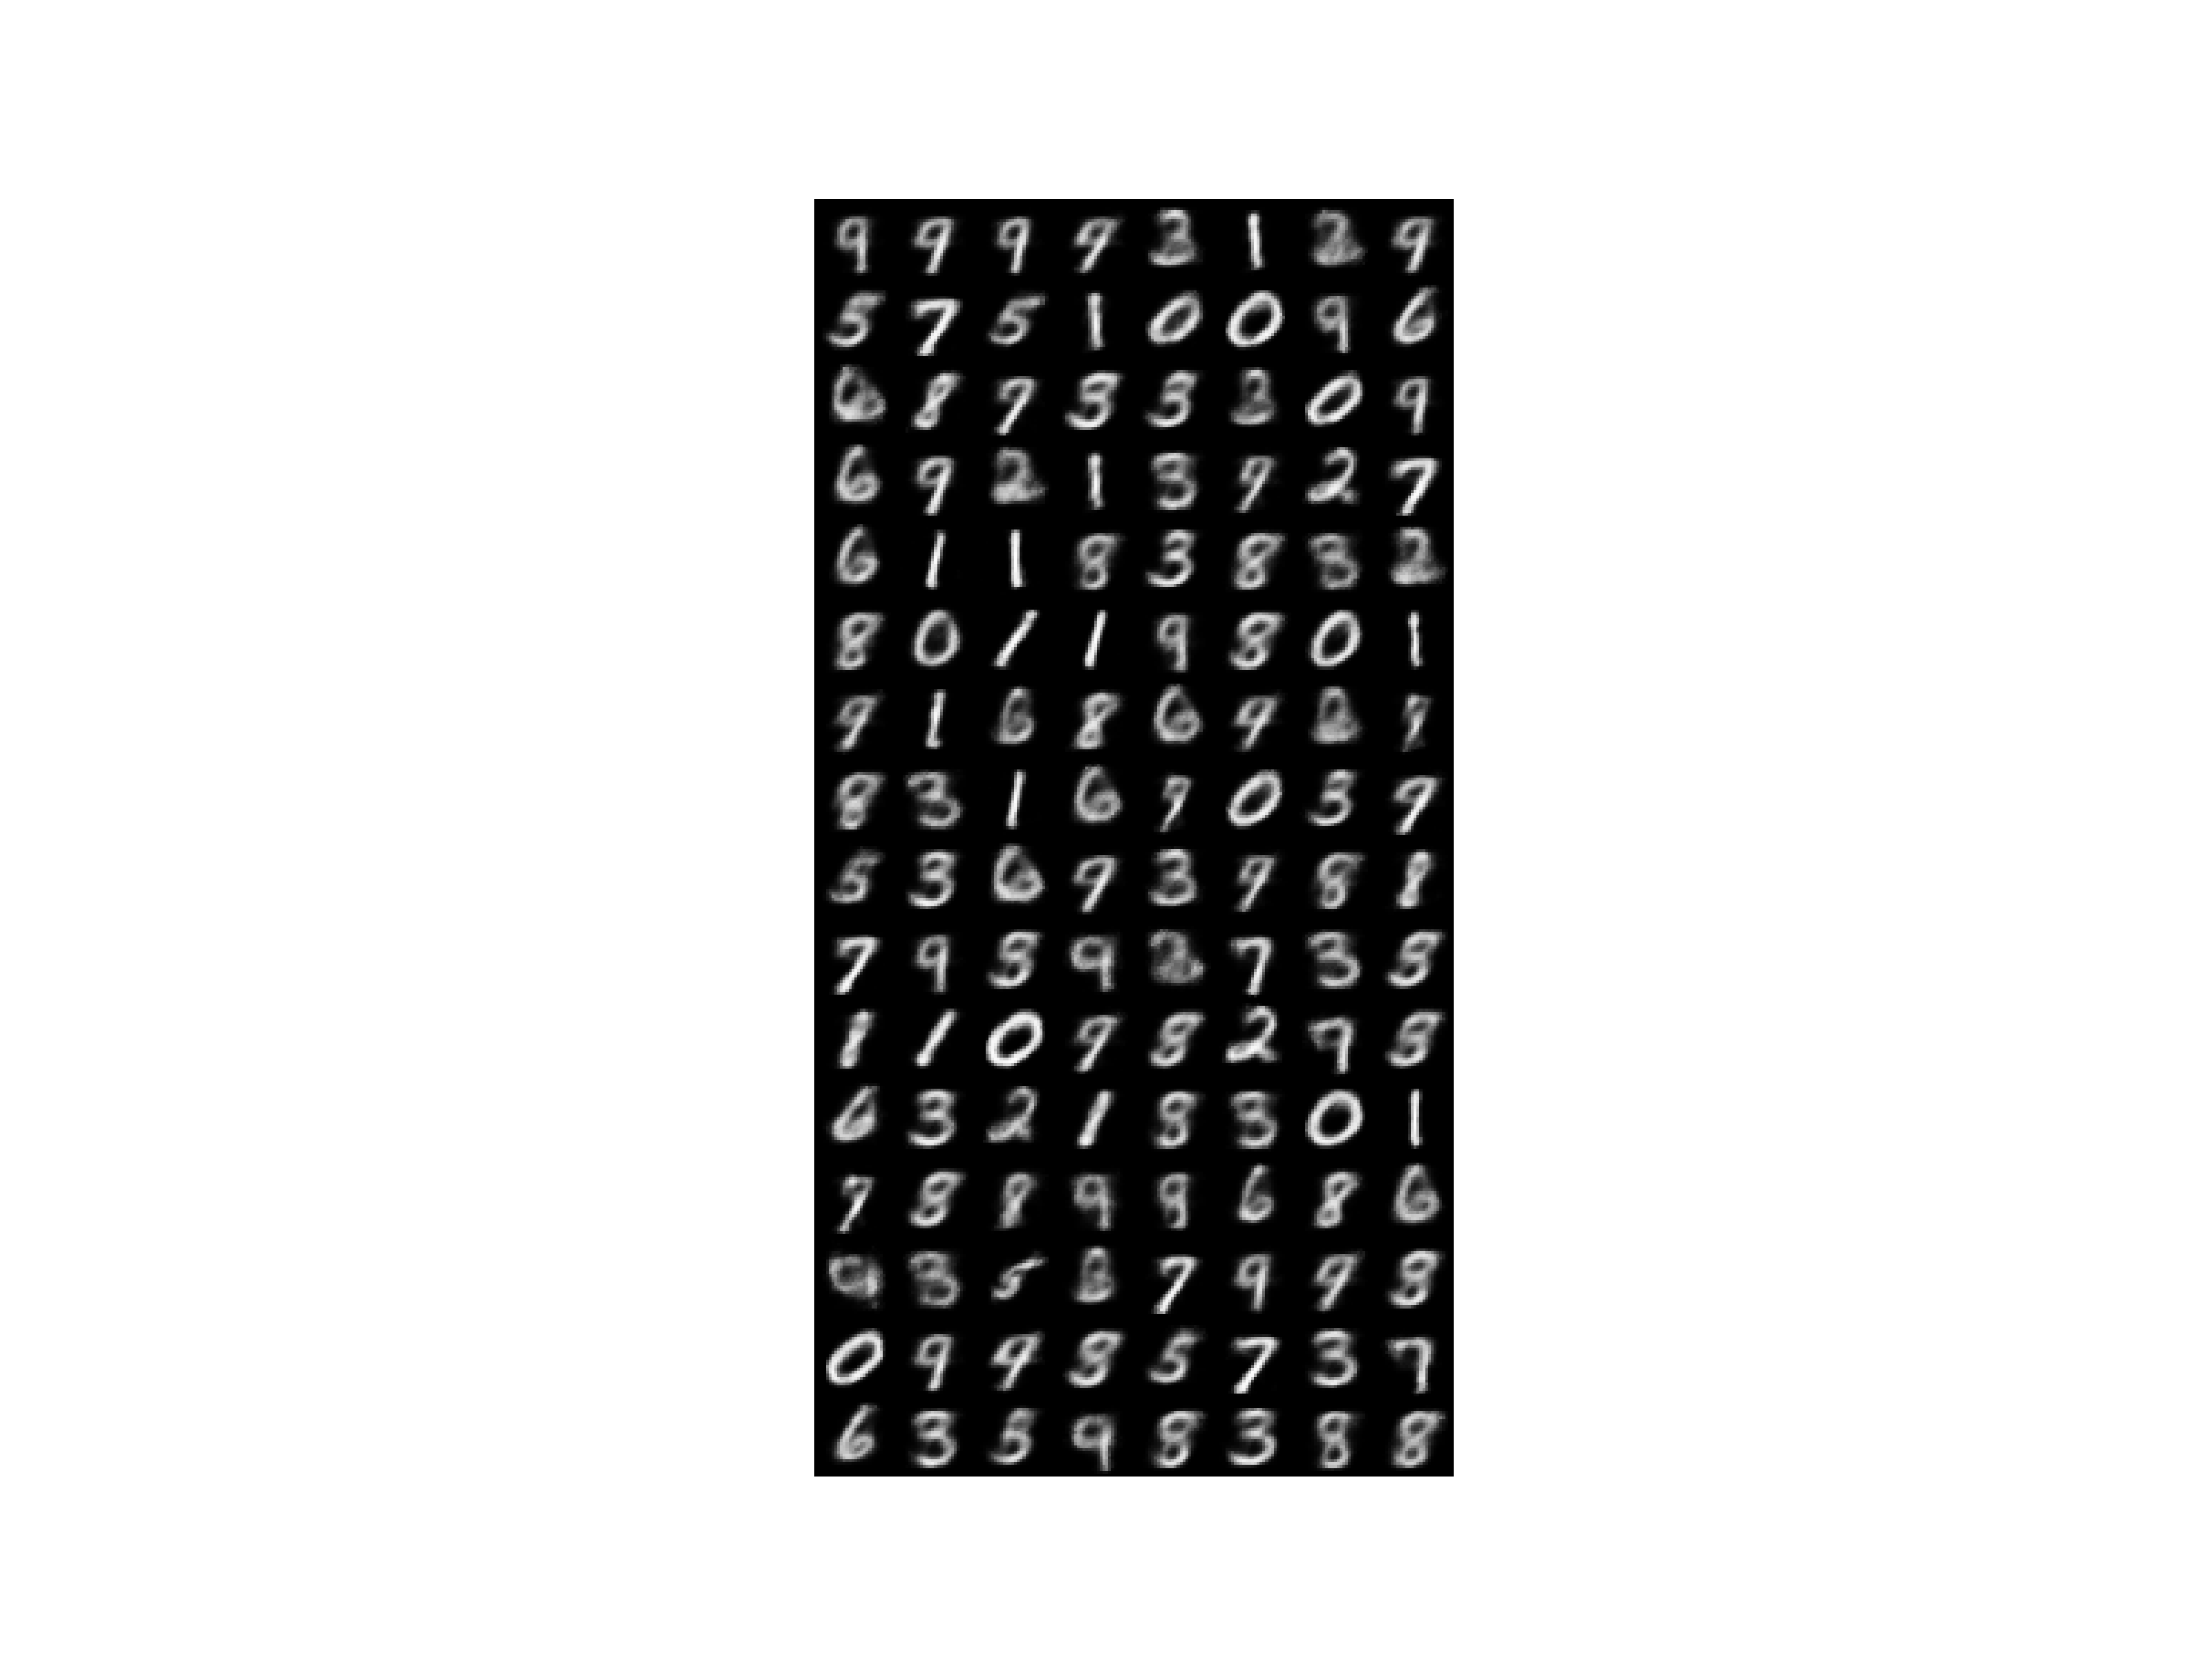
\includegraphics[width=0.3\linewidth]{plt5.png}
            }
            \subfloat[][n = 100]{
                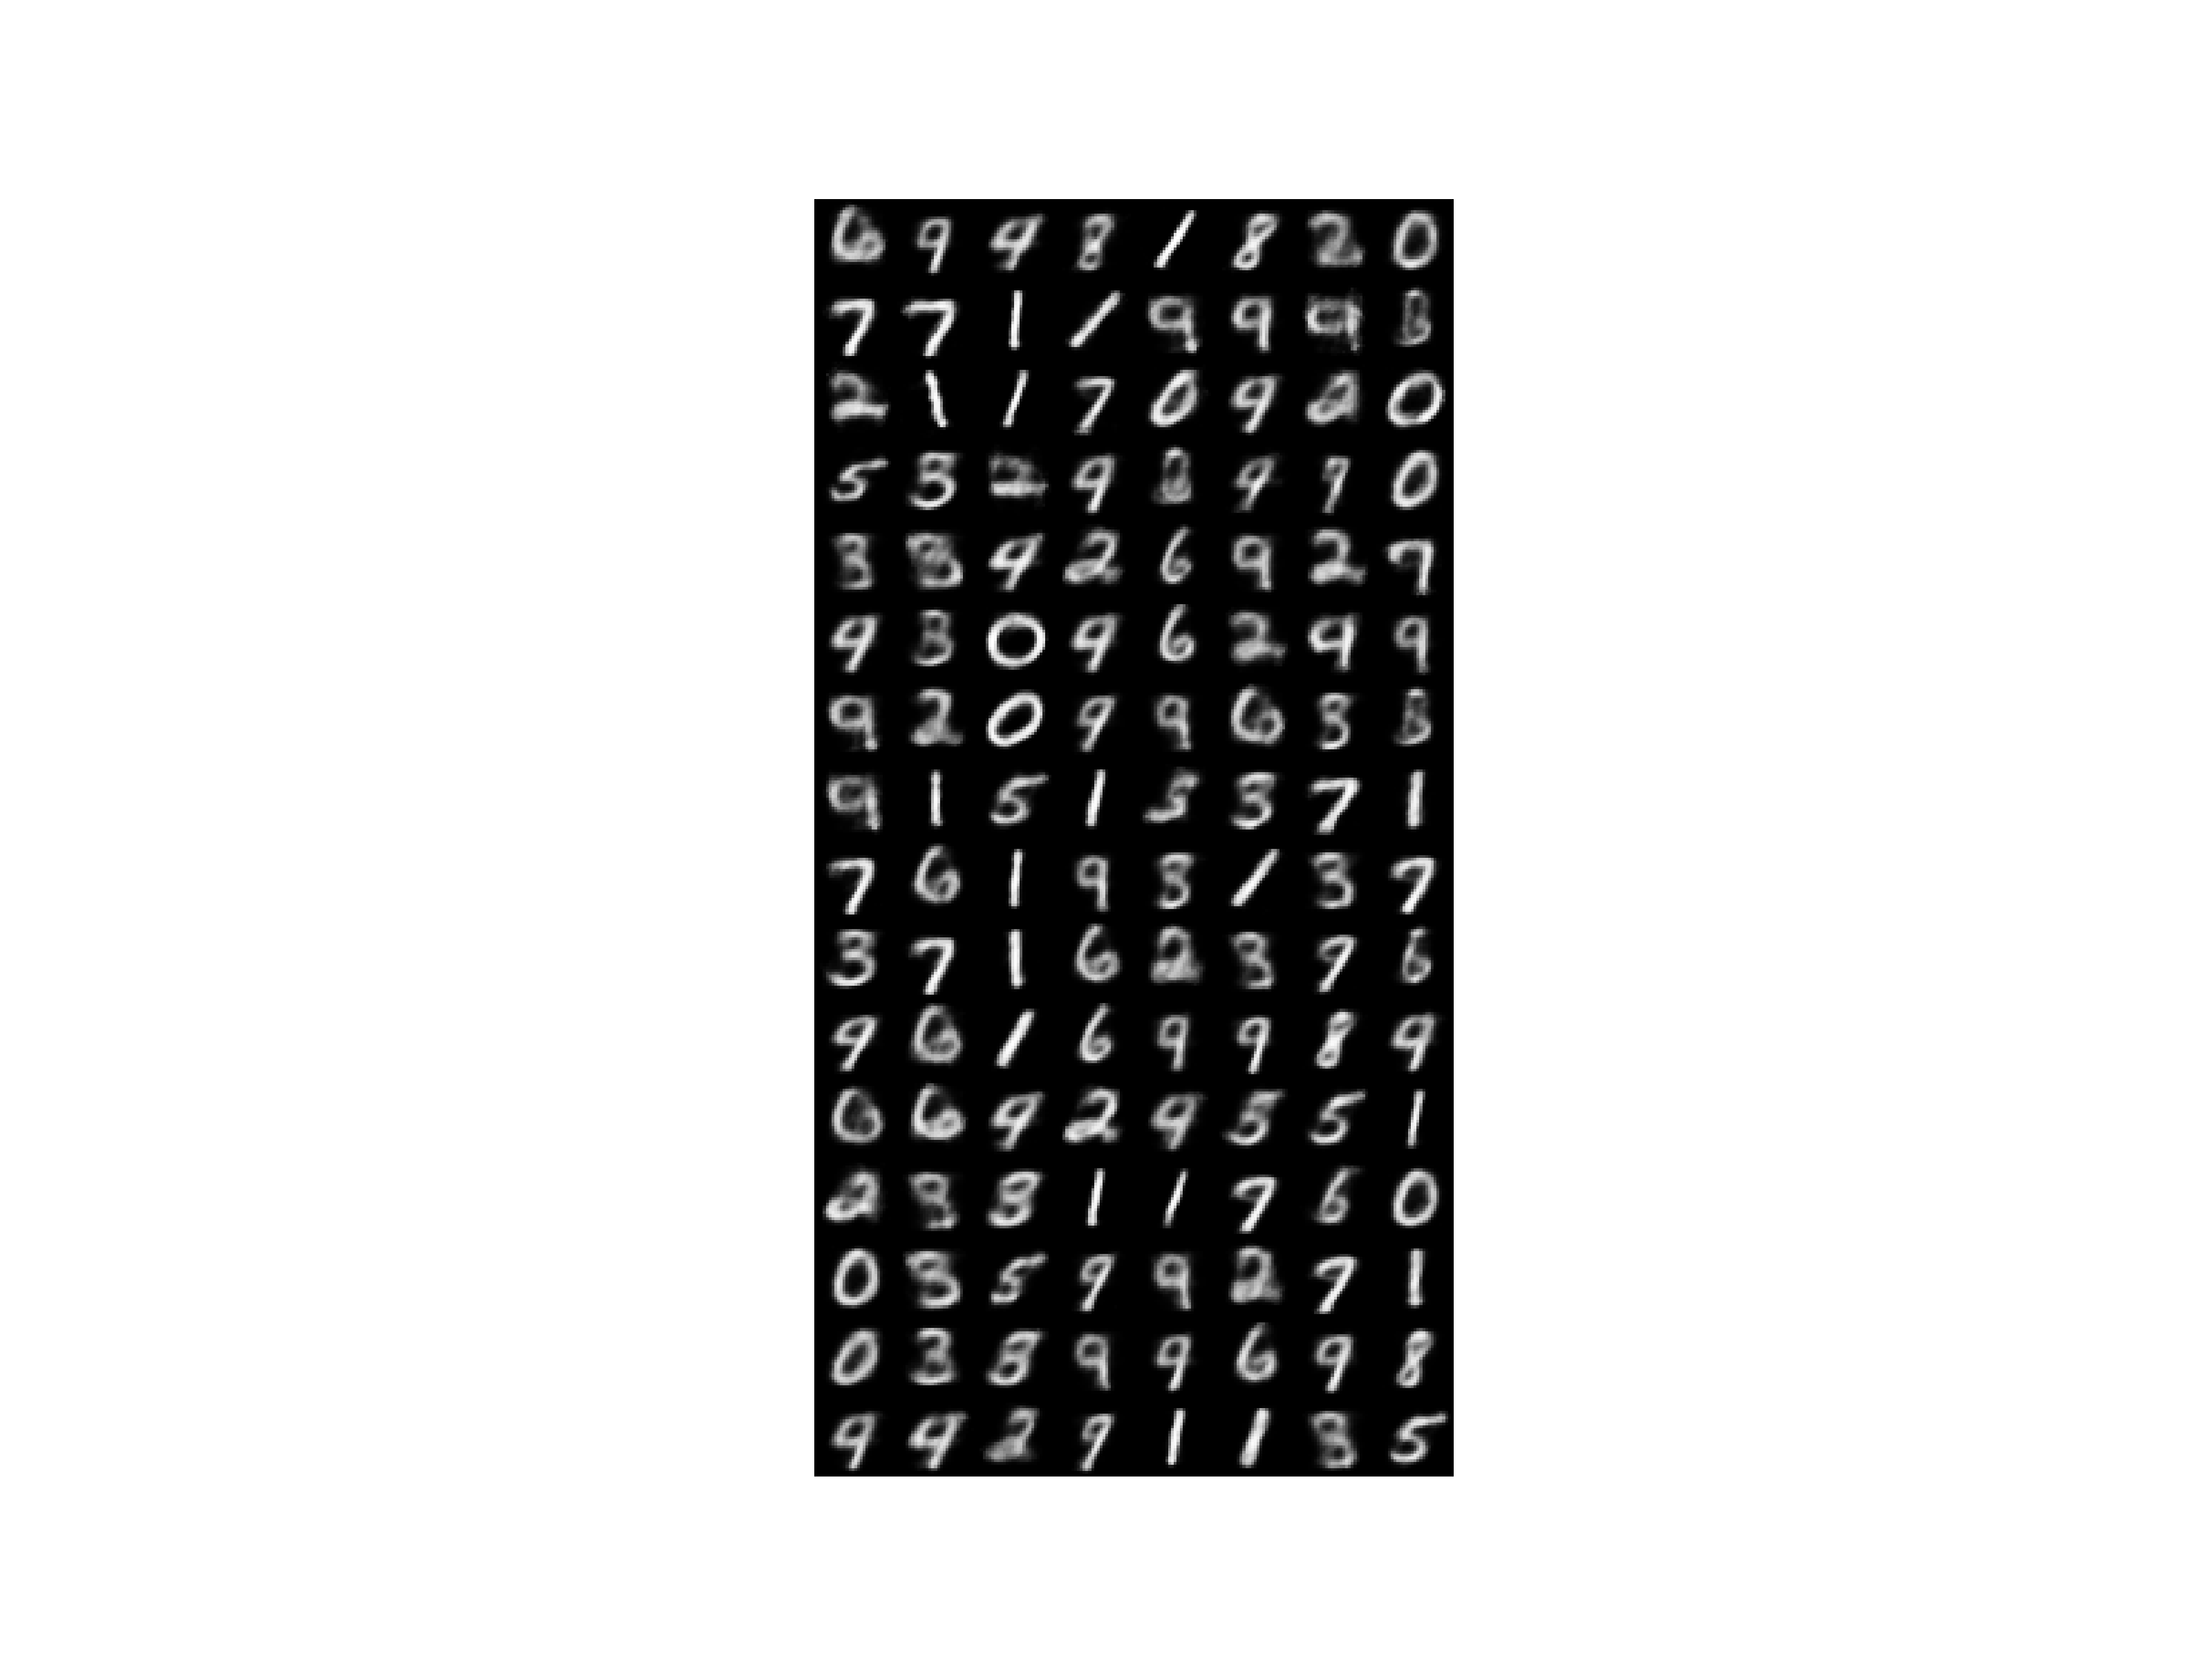
\includegraphics[width=0.3\linewidth]{plt10.png}
            }
            \caption{Results of VAE after n iterations.}
            \label{fig:q10}
        \end{figure}
        \par The results for this are shown in figure ~\ref{fig:q10}.


    % % Now we need a bibliography:
    \begin{thebibliography}{1}
    
        % %Each item starts with a \bibitem{reference} command and the details thereafter.
        \bibitem{carl} % Transaction paper
        C.~Henrik ~Ek,  Machine Learning Lecture Series\\
        Autumn 2017. \\
        \url{https://github.com/carlhenrikek/COMS30007}

        \bibitem{inftheory} % Transaction paper
        F. ~Bavaud,  Relative Entropy and Statistics\\
        Apr 2010.
    
    \end{thebibliography}
    
    % Your document ends here!
    \end{document}